\section{Reminder on Schemes}

The basic building blocks of algebraic geometry are affine schemes. An affine scheme $\Spec(A)$ is a geometric object constructed out of the prime spectrum 
\[
  \{p \subseteq A \mid p \text{ prime ideal}\}
\]
of a commutative ring $A$. This set is equipped with a topology generated by sets of the form 
\begin{align*}
  D_f &= \{ p \in \Spec(A) \mid f \not \subseteq p \} \\
      &= \{ p \in \Spec(A) \mid f(p) \neq 0\} .
\end{align*}
The closed sets of $\Spec(A)$ are thus of the form
\begin{align*}
  V_f &= \{ p \in \Spec(A) \mid f \subseteq p \} \\
      &= \{ p \in \Spec(A) \mid f(p) = 0\} ,
\end{align*}
the vanishing set or zero locus of $f$. Here $f(p)$ is defined to be the image of $f$ under the quotient map $A \to A/p$. The notation indicates that we interpret the elements $f \in A$ as functions on the space $\Spec(A)$. Since $f(p) \neq 0$ for all $p \in D_f$, we view the the ring $A[1/f]$ as the ring of rational functions defined on $D_f$. It consists of elements of the form 
\[
  \biggl\{ \frac{g}{f^k} \mid g \in A, k \in \N \biggr\}.
\]
The association $D_f \to A[1/f]$ extends to a presheaf $\Sh{O}_{\Spec{A}}: \Spec(A) \to \mathsf{Ring}$.
This presheaf is in fact a sheaf. This sheaf has the property that all stalks are local rings. We obtain a fully faithful functor
\[
\Spec : \text{CRing} \to LRS
\]
from the category of commutative rings to the category of locally ringed spaces. The category of schemes now consists of spaces which are locally affine. We would like to apply methods from algebraic to these geometric spaces. However, the Zariski topology on a scheme $X$ is inadequate for a number of geometric constructions:

\begin{itemize}
  \item There is no universal covering space.
        For instance, the algebra-morphism given by $x^n \to x^n, k[x^n] \to k[x]$ corresponds to a map $x \to x^n, \mathbb{A}^1_k \to \mathbb{A}^1_k$. Depicted is the map from $\mathbb{A}^1_\mathbb{C}$ to $\mathbb{A}^1_\mathbb{C}$ for the case $n=2$
        \begin{center}
          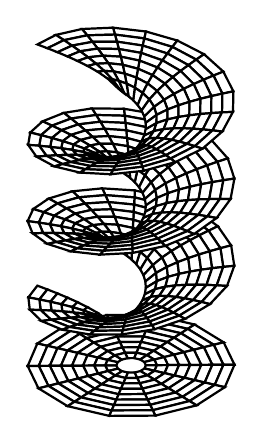
\begin{tikzpicture}[scale=2]
    \begin{axis}[
        axis lines=none,
        axis equal image,
        trig format plots=rad,
        z buffer=sort]
   \addplot3 [
        surf,
        domain=1:7,
        domain y=-pi:pi,
        samples=9,
        samples y=15,
        shader=flat,
        draw=black,
        fill=white
        ]
    ({x*cos(y)},{x*sin(y)},{-12});
   \addplot3 [
        surf,
        domain=1:7,
        samples=9,
        samples y=60,
        shader=flat,
        draw=black,
        fill=white,
        domain y=-3*pi:3*pi
        ]
    ({x*cos(y)},{x*sin(y)},{ln(x)+ y});
    \end{axis}
  \end{tikzpicture}



          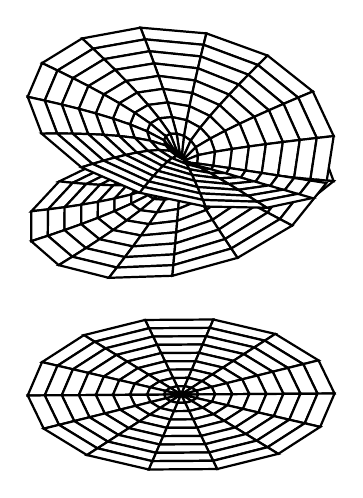
\begin{tikzpicture}[scale=2]
  \begin{axis}[
    axis equal image,
    axis lines=none,
    trig format plots=rad,
    z buffer=sort,
  ]

  \addplot3 [
    surf,
    domain=0:2*pi,
    samples=15,
    y domain =0:4,
    samples y=10,
    shader=flat,
    draw=black,
    fill=white,
  ]
  ({y*cos(x)}, {y*sin(x)}, {-7});

  \addplot3 [
    surf,
    shader=flat,
    draw=black,
    fill=white,
    z buffer=sort,
    domain=pi:5*pi,
    y domain = 0:4,
    samples = 30,
    samples y=10,
    ] 
  ({y*cos(x)}, {y*sin(x)}, {sqrt(y)*sin(x/2)});

  \end{axis}
  \end{tikzpicture}



        \end{center}
        This map \textit{should} be local homeomorphism, but this is false in the Zariski topology. There do not exist nonempty open subsets $V$ and $U$ such that $x \to x^n$ maps $V$ isomorphically onto $U$.
  \item fibre bundles aren't locally trivial.
\end{itemize}
  
These issues all stem from the fact that the Zariski topology is very coarse.  Grothendieck found a natural generalisation of the notion of topology, allowing not only open subsets $U \subseteq X$ but more generally morphisms of schemes $Y \to X$ to play the role of open set. Specifically, he defined the \textit{\'etale site of $X$}, a generalised topology on $X$, consisting of the following:


\begin{itemize}
  \item The category of \'etale schemes $\text{\'Et}/X$ over $X$. This category consists of schemes $S$ together with an \'etale morphism $f: S \to X$. These morphisms formally behave like local homeomorphisms. 
  \item A notion of covering. In this case a covering of $X$ is a family of morphisms $\{\varphi_i: U_i \to X\}$ such that they are jointly surjective, $\bigcup_i im(\varphi_i) = X$. We will make this more precise later.
\end{itemize}

The \'etale topos $\mathsf{Sh}(X)$ of a scheme $X$ is the category of sheaves on the \'etale site of $X$.  The \'etale topos $\mathsf{Sh}(X)$ may be thought of as a generalised space, locally modeled on $X$, with a close relation to the geometric properties of $X$. 

Because \'etale morphisms behave like local homeomorphisms, it is possible to realise the theory of covering spaces for schemes. In particular this means that we get a good notion the fundamental groups $\pi_1(X)$. Furthermore, the \'etale topos $\mathsf{Sh}(X)$ also allows us to compute cohomology for sheaves which have vanishing cohomology in the Zariski setting. In this sense the \'etale site of a scheme is a much finer topology than the Zariski topology. 

%A locally ringed space is a pair $(X, \mathcal{O}_X)$ where $X$ is a topological space and $\mathcal{O}_X$ is a sheaf of rings on $X$, such that all stalks $\mathcal{O}_{X,x}$ are local rings. There is a functor \[\mathsf{CommR} \to \mathsf{LRS}\]
%A scheme is in particular a locally ringed space, meaning it comes equipped with a sheaf of rings such that the stalks are local rings. This has some important consequences for the theory of schemes. If we wish to take seriously the \'etale topology as a replacement for the Zariski topology, these consequences should have analogues in the \'etale setting as well.
%
%For a sheaf of rings $\mathcal{F}$, the stalk of $\mathcal{F}$ at $x \in X$ is defined to be $\colim F(U)$, where $U$ runs over all neighborhoods of $x$. This group captures the local behavior of $\mathcal{F}$ around $x$. For this definition to make sense in the \'etale setting, we need to verify that the category of \'etale neighborhoods at $x$ is cofiltered.k
%
%\section{A brief Reminder on Schemes}
%The starting point of modern algebraic geometry is the definition of affine schemes. We briefly recall the definition and its most important consequences, after which we will construct their analogues in the \'etale setting.
%
%Let $A$ be a ring. The spectrum of $A$ is the set $\{\mathfrak{p} \subseteq A | \mathfrak{p} \text{ prime ideal}\}$. For any ideal $\mathfrak{a}$ of $A$ we write $V(\mathfrak{a})$ for the set of prime ideals containing $\mathfrak{a}$. By basic algebra one may deduce that the sets $V(\mathfrak{a})$ form the closed sets of a topology on $\Spec A$. 
%%Affine schemes are locally ringed spaces constructed from commutative rings. We briefly recall the construction. Let $A$ be a commutative ring. We put a topology on the set of prime ideals of $A$. 
%%$\{\mathfrak{p} \subseteq A | \mathfrak{p} \text{ prime }\}$
%
%
%Schemes are locally ringed spaces that are locally affine.
%Now that we have available the \'etale topology for a scheme


\subsection{Interpretation of Cohomology}
Cohomology groups are not just of interest in their own right. In many cases, one can show that the cohomology classes $[\gamma] \in H^n(X, \Sh{A})$ correspond bijectively to some other kind of geometrical construction involving $X$.

For instance, when $p:Z \to B$ is a map of topological spaces and $\Sh{G}$  is a sheaf of subgroups of $Aut_B(Z)$, one can define a notion of “twist of $p$ with structure sheaf $\Sh{G}$”. One obtains the bijection
\begin{align}
            \left\{ \parbox[c]{1.1in}{\centering
                       Isomorphism classes of twists of $p$
                       with structure sheaf $\Sh{G}$}
            \right\}
            \stackrel{\sim}{\to}
            \parbox[c]{0.5in}{\centering
                       $H^1(B, \Sh{G})$}
\end{align}

There is also a bijection
\begin{align}
            \left\{ \parbox[c]{1.1in}{\centering
              Isomorphism classes of vector bundles of rank $n$ with basis $B$}
            \right\}
            \stackrel{\sim}{\to}
            \parbox[c]{0.5in}{\centering
            $H^1(B, GL_{n,B})$}
\end{align}
and in particular
\begin{align}
            \left\{ \parbox[c]{1.1in}{\centering
            Isomorphism classes of line bundles with basis $B$}
            \right\}
            \stackrel{\sim}{\to}
            \parbox[c]{0.5in}{\centering
                $H^1(B, \Ring(O)_B^\times)$}
\end{align}


\begin{figure}[h]
\centering
\subimport{introduction/}{mobius.tex}
\caption{The gluing data of the mobius strip.}
\end{figure}


\section{The \'etale topology}
The natural topology one has available in algebraic geometry is the Zariski topology. For some purposes this topology is insufficient. In particular, by a theorem of Grothendieck, higher cohomology for constant sheaves vanishes, so we can not use sheaf cohomology to define Betti numbers. The reason is that the open sets of the Zariski topology are very large. However, instead of considering Zariski-open sets, one may use the notion of \'etale open sets. These are not really open sets of a topological space, but formally share many properties of open sets. In particular, they have all the properties one needs to define sheaves and their cohomology. This, in turn, yields satisfactory analogues from algebraic topology. 

\section{prerequisites}
We assume aqcuaintance with the basics of category theory including limits and adjoint functors. We will make free use of results from algebra but will provide references wherever needed. We will also use basic notions of scheme theory.

%\section{WIP}
%Another central notion of modern geometry is that one thinks of spaces as being “glued together” from simple building blocks. A manifold is locally modelled on $\mathbb{R}^n$. A simplicial complex and more generally simplicial sets and simplicial objects are geometric objects that are modeled on the standard simplices $\Delta^n$, depicted below for $n = 1,2,3$.
%
%% missing figure
%
%Because a manifold $X$ is locally modelled on euclidian space, it comes equipped with a so-called sheaf of of rings $\Sh{O}_X$, which is inherited from the ring structure on $\R$. In particular there is the ring of \textit{global} sections
%\[\{f: X \to \R \} \coloneqq  \Gamma(\Sh{O}, X).\]
%Can we interpret an arbitrary commutative ring as a ring of functions on a geometric object?
%Alexander Grothendieck's definition of schemes provide an answer: For any ring $R$ there is a locally ringed space $(X, \Sh{O}_X) = (\Spec(R), \Sh{O}_{\Spec(R)})$ such that $\Gamma(X, \Sh{O}_X) \cong R$
%